%---------------- COMMENT FOR IMPORTING ----------------------
%\RequirePackage{lineno}					%Comment for importing
%\documentclass[12pt]{report}		%Comment for importing
%\pagestyle{headings}
%\input{ST-input2}								%Comment for importing

%\setcounter{chapter}{2}
%\begin{document}								%Comment for importing
%\setpagewiselinenumbers
%\linenumbers
%\tableofcontents
\graphicspath{{Chapter4/figures/}} 
%-------------------------------------------------------------

\chapter{The Effect of Recovery Algorithms on Compressive Sensing Background Subtraction}
\label{chap:CSBGS}

\textit{This chapter appears in the form of a conference paper \citep{Davies2013}. Supplementary material is provided in Appendix \ref{chap:ap_B}. This material includes a broader introduction to compressive sensing, a description of the conditions for choosing a stable measurement matrix and  intuition for the orthogonal matching pursuit algorithm.}\\

 %\begin{center}
%  \textbf{Abstract}
%\end{center}
%\begin{abstract}
%\boldmath

Background subtraction is a key method required to aid processing surveillance videos. Current methods require storing each pixel of every video frame, which can be wasteful as most of this information refers to the uninteresting background. 

Compressive sensing can offer an efficient solution by using the fact that foreground is often sparse in the spatial domain. By making this assumption and applying a specific recovery algorithm to a trained background, it is possible to reconstruct the foreground, using only a low dimensional representation of the difference between the current frame and the estimated background scene. 

Although new compressive sensing background subtraction algorithms are being created, no study has been made of the effect of recovery algorithms on performance of background subtraction. This is considered by applying both basis pursuit and orthogonal matching pursuit (OMP) to a standard test video, and comparing their accuracy. 

% Current methods for this are inefficient as most of the time, we observe background which is not important or of interest. We wish to be able to have information as to the location of foreground in a frame, without having to store information about every individual pixel in every single frame as this can be computationally heavy. 
%\end{abstract}


\section{Introduction}
Surveillance cameras have become ubiquitous in many countries, constantly collecting a huge amount of data most of which is stored and never analysed. This is due to the challenge of converting a large volume of video data into useful information, particularly as several cameras may be acquiring data simultaneously. One of the main aims of collecting surveillance footage is to track an object or classify its behaviour, therefore the first step in video analysis is to identify the objects of interest from the background.

%  An automatic detection system could be used to notify the user of unusual behaviour in a place of interest, such as someone placing a package and leaving it in a busy areas or putting goods into their bag, or it could be used to highlight activity in an unusual place at an unusual time, for example a person walking through a private area in the middle of the night.

Background subtraction \citep{Piccardi2004a} is a method used to separate the foreground from the background of a video sequence. This consists of constructing and updating a model of the background and then subtracting it from the current frame. Background subtraction is not a new development and many methods for modelling a background scene exist, however traditional background subtraction methods are not very efficient. Most surveillance footage consists of a slowly adapting background scene with foreground appearing in a subset of the frames and when foreground does appear in the footage it usually takes up only a small percentage of the overall frame. Traditional background subtraction methods require that all pixels are acquired for each frame in order to correctly segment the two layers, however since foreground is sparse in most surveillance footage this can be seen as a waste of resources. 

In order to combat this inefficiency, the single pixel camera (SPC) \citep{Duarte2008Single} was developed; a camera based on the theory of compressive sensing \citep{Candes2006, Candes2006a, Donoho2006} and designed to acquire images directly in compressed format. Once surveillance footage is acquired using a camera such as the SPC, background subtraction can be performed on this low dimensional representation of the video frames. Later a recovery algorithm is used to decode a mask of the foreground into the correct dimension. The reason for using this technique is, due to the natural sparsity property of foreground, a mask can be reconstructed without ever storing the current frame, or background model in the full dimensional form. The computational savings available are significant, provided that the segmentation performed is accurate enough for the purpose of the application. 
% When compressive sensing is applied to surveillance footage, the video is encoded into a lower dimension,

This paper discusses if the choice of recovery algorithm affects the performance of compressive sensing background subtraction. In particular two algorithms are investigated, basis pursuit \citep{Candes2005} which is an algorithm based on convex optimisation \citep{boyd2004convex} and a greedy algorithm called orthogonal matching pursuit \citep{Tropp2004}. Results are presented from both algorithms on data which was gathered using a conventional camera but which have been simulated to mimic the acquisition process of compressive sensing imaging technology such as the SPC. 

The rest of this paper is organised as follows; Section \ref{sec:related-works} discusses the related works in this area in brief before discussing the methodology behind compressive sensing and its application to background subtraction in Section \ref{sec:background}. Experimentation is conducted in Section \ref{sec:results} and conclusions are given in Section \ref{sec:conclusions}. 

% Compressive sensing  can improve on the efficiency of segmentation algorithms by incorporating this foreground sparsity feature into the background subtraction process.

\section{Related Works}
\label{sec:related-works}

There is a vast amount of research available  in the literature detailing the many techniques for background subtraction; notable comparative studies include \cite{Sen-Ching2004} and \cite{Piccardi2004a}. Generally, algorithms for background modelling  can be categorised into pixel based and region based methods  \citep{Bouwmans2011}. The latter may seem more intuitive as one expects foreground to be clustered and generally not exist as isolated pixels. Using knowledge of neighbouring pixels should therefore improve the classification of pixels into foreground or background, and region based techniques such as  \cite{elgammal2000} and \cite{toyama1999} do use this knowledge to segment the images into regions and then create a background model based on these regions. However, there are downsides to region based techniques, for example they are often a lot more complex to run than pixel based techniques, and are not generally robust to division of blocks.

Pixel-based methods such as approximate median filtering \citep{McFarlane1995} assume that the pixels observed are classified as foreground independently of each other. These methods can often detect the contours of foreground well but may be susceptible to making false classifications, especially if the background model is not well tuned.  

It is also possible to categorise these algorithms as recursive and non-recursive methods \citep{Bouwmans2011}. A non-recursive algorithm maintains a buffer or window of $N$ previous video frames and estimates a background model based on the statistical properties of these frames. This sliding window is usually required to be fairly large in order to obtain accurate results, and therefore can quickly become computationally intensive. Recursive techniques update the background subtraction each time a new frame is stored and so there is no need to buffer previous frames. The method used in Section \ref{sec:backgr-subtr-with} to model the background is a pixel-based, recursive method.

More recently the new technology of compressive sensing \citep{Candes2006, Candes2006a, Donoho2006} has been applied to the background subtraction problem. The theory of compressed sensing states that an under-sampled signal can be recovered almost perfectly, given that the signal itself is sparse in some domain \citep{Baraniuk2007}, i.e. a large proportion of the signal's elements are close to zero. In compressive sensing for video, a random matrix is used to encode a signal efficiently, and then a recovery algorithm is used to decode the signal and recover the required information fairly accurately. 

Most compressed sensing background subtraction methods \citep{Cevher2008a, Cevher2008b, Warnell2011, Cossalter2009} make the assumption that the majority of the pixels in a video represent the background, and therefore the foreground is sparse in the spatial domain. This key point allows us to encode a video into a low dimension and then search for a sparse solution, using the knowledge that the foreground mask should be suitably sparse. 

The background subtraction problem is first expressed as a sparse signal recovery problem in \cite{Cevher2008b}. Their work successfully recovers silhouettes of foreground activity by modelling a compressed form of the background and recovering a foreground mask directly from compressed measurements. Later \cite{Warnell2011} builds upon this work by proposing a method that adapts the encoding process between frames to incorporate the changing size of foreground. Unlike \cite{Cevher2008b}, \cite{Warnell2011} choose to use a static model for the background which could cause problems in the model when applying to real-life video. 

More current work has started attempting to incorporate the structure of foreground into segmentation. It is generally expected that foreground will be clustered into particular shapes in most frames and does not consist of isolated pixels. Foreground often consists of humans, animals and vehicles, and so knowledge of this structure could be used to improve segmentation. Currently many different approaches are being investigated such as applying particle filters \citep{Cossalter2009} and lattice based graphical models \citep{Cevher2008a}. Although cluster type methods are not attempted in this work, it is a research area of interest for future investigation. 

%\cite{Qiu2012} have developed a robust recursive PCA type method to seperate foreground and Background. They use PCA to identify the 'outlier' (the foreground) from the low dimensional subspace (background.) Their algorithm entitlted ReProCs is online, and uses deails about the previous foreground to help vpredict the location of the current foreground by taking advatage of the clustering of foreground. This would fail if the foreground appeared from the centre of the image. 

%\cite{Cossalter2009} keeps tracks of object of interest by applying particle filters to the compressed frames, without ever reconstructing the original image (I.E background subtraction is applied during the the projection domain. The SPGL1 algorithm is applied to recover he foreground and the background is modelled in a block based framework. 

%\cite{Liu2010} focusses on a block based approach, which focuses on using inter-frame correlation. One issue that arrises from this technique is that different regions of the image may exhibt different types of inter-frame correlation. Their method reconstructs the entire image and then applies techniques which is inefficient. But they do instigate a foreground detection which is a threshold based method for determining if there exists foreground in the current frame or not.  

%\cite{Lu2010} discusses alot of the literature based on combining CS with tracking type algorithms but does not focus on the efficiency of assuming the staparsity of foreground in the spatial domain. 

%\cite{Zhao2011}bases their work on the assution that the background has a sparse lienar representation over learned dictionary and that the foreground is sparse.  

%Sparse coding based visual tracking
%Has an emphasis on tracking algorithms
%Good discussion or why sparse coding is of value to visual tracking, and if it helps atall. 

%\cite{Cevher2008a}The foreground is often clustered aswell as sparse. We expect foreground to take the shape of a car/vehicle or a person or an animal. Obsiouly this depends on the video we are duscussing but certain could be universal in sandard surveillance footage. (FOOTAGE is all so different / similar). 

%\cite{Li2011} choses to uses hash kernels instead of a random measurement to acquire their signal. Their algorithm uses a customised orthogonal matching pursuit to track foreground. Uses background templates and evalutates all work in terms of the TSP. 

In this work, two recovery algorithms are compared, one greedy method and one based on convex optimisation when applied to a background subtraction algorithm. 
%The proposed work is inspired by \cite{Cevher2008b}, we wish to be able to understand the effects of different recovery algorithms on the performance of background subtraction, and how the sparsity of the real footage can affect the performance of such algorithms. 

%In summary the main contributions made in this paper are: 
%\begin{itemize}
%\item A comparison of recovery algorithms in a compressive sensing for background subtraction setting. 
%\item Better understanding of the effect of sparsity in foreground detection.
%\item Discussion of the advantages of using sparsity properties in video analysis.
%\end{itemize}

\section{Methodology}
\label{sec:background}

In this section, the main theory is introduced, starting with the explanation of sparse signals in Section \ref{sec:compressible-signals}, progressing to the theory of compressive sensing in Section \ref{sec:compressive-sensing} with a focus on the two recovery algorithms of interest in Section \ref{sec:recovery-algorithms} and finally notes on applying this theory to the background subtraction problem in Section \ref{sec:backgr-subtr-with}.

\subsection{Sparse and Compressible Signals}

\label{sec:compressible-signals}
A signal is known as being $K$-sparse if $\boldsymbol{x} \in R^N$ can be represented as a linear combination of $K$ basis vectors \citep{Baraniuk2007}. The case of interest occurs when $K$ is much smaller than $N$ as this means that most of the coefficients are zero. No signal is ever truly sparse in the presence of noise and so some signals are described as approximately sparse, or compressible. If a signal is compressible there exist $K$ large coefficients (with $K \ll N$) but the remaining $N-K$ coefficients are only required to be small and not necessarily zero. Fundamentally a signal is compressible if most of the information in the signal is represented by a few coefficients.

\subsection{Compressive Sensing}
\label{sec:compressive-sensing}

According to the framework developed in \cite{Candes2006},  \cite{Candes2006a} and \cite{Donoho2006}, the measurement $\boldsymbol{y}$ is a linear function of the signal $\boldsymbol{x}$ as shown in equation \eqref{eq:ch4_BIG}. The number of measurements $M$ in $\boldsymbol{y}$ is chosen to be smaller than $N$, so a measurement matrix $\boldsymbol{\Phi} \in R^{M \times N}$ is chosen, with $M \ll N$. Although it is known from linear algebra that there are infinitely many vectors $\boldsymbol{x}$ that can solve equation \eqref{eq:ch4_BIG}, the knowledge that the original signal $\boldsymbol{x}$ was sparse can be used to help the reconstruction process, given that certain conditions hold for $\boldsymbol{\Phi}$. 

%It is known from linear algebra that there are infinitely many vectors $\boldsymbol{x}$ that can solve Eq. \eqref{eq:10}, but usually $\boldsymbol{x}$ is the only sparse solution, provided that $M \geq 2K$, where $K$ is the true sparsity of the signal. Therefore if $\boldsymbol{x}$ is known in advance to be sparse, it can in theory be reconstructed exactly from $M$ measurements.
%
\begin{equation}
  \label{eq:ch4_BIG}
\boldsymbol{y} =\boldsymbol{\Phi x}.
\end{equation}
%% Assuming that $\boldsymbol{x}$ is $K$-sparse, and that the location of these $K$ large coefficients is known, it is possible to reconstruct $\boldsymbol{x}$ accurately for $M > K \log N$, but a number of conditions must be true of the measurement matrix $\boldsymbol{\Phi}$.. $\boldsymbol{\Phi}$ needs to enable the signal $\boldsymbol{x} \in R^N$ to be be reconstructed accurately from the measurement vector $\boldsymbol{y} \in R^M$.
It is of vital importance that a stable measurement matrix $\boldsymbol{\Phi}$ is designed so that the signal information is not damaged by the dimensional reduction from $\boldsymbol{x} \in R^N$ to $\boldsymbol{y} \in R^M$. In order for the reconstruction problem to be well-conditioned, it is sufficient that ${\boldsymbol{\Phi}}$ holds the Restricted Isometry Property (RIP) \citep{Donoho2006} of order $2K$. 

\begin{mydef}
 A matrix $\boldsymbol{\Phi}$ satisfies the (RIP) of order $K$ if there exists a $\delta_K  \in (0,1)$ such that 
\begin{equation*}
  \label{eq:401}
  (1 - \delta_k)\|\boldsymbol{x}\|^2_2 \leq\|\boldsymbol{\Phi} \boldsymbol{x}\|^2_2 \leq (1 + \delta_k)\|\boldsymbol{x}\|^2_2,
\end{equation*}

for all $\boldsymbol{x} \in \sum_K = \{\boldsymbol{x}:\|\boldsymbol{x}\|_0 \leq K\} $, \newline

where $\|\boldsymbol{x}\|_0$ is the zero pseudo-norm defined as

\begin{equation*}
\|\boldsymbol{x}\|_0 = \#(i|x_i \neq 0). 
\end{equation*}
 
\end{mydef}

%WRONG?
%The $l_2$ norm is defined  in equation \eqref{eq:573}. 
%
%\begin{equation}
%\label{eq:573}
%  ||\boldsymbol{x}||_2 = \sum_{i=1}^{N}||\boldsymbol{x_i}^2||
%\end{equation}

If $\boldsymbol{\Phi}$ satisfies the RIP with order $2K$, then $\boldsymbol{\Phi}$ approximately preserves the distance between any pair of $K$-sparse vectors. Unfortunately the task of checking that a matrix satisfies the RIP is a NP-hard problem, but fortunately the RIP will hold true with high probability if $\boldsymbol{\Phi}$ is selected as a random matrix \citep{Candes2006a}, and $M \geq cK\log \frac{N}{K}$, where $c$ is a small constant. 

%Another essential condition when selecting a $\Phi$ is incoherence, which requires that the rows of $\boldsymbol{\Phi}$ cannot sparsely represent the columns of $\boldsymbol{\Psi}$, and vice versa the the rows of $\boldsymbol{\Psi}$ cannot sparsely represent the columns of $\boldsymbol{\Phi}$, which will ensure that $\boldsymbol{\hat{x}}$ is a unique solution.
%In order to construct $\boldsymbol{\Phi}$ as such, we choose the entries $\phi_{i,j}$ as independent realisations of some probability distribution.
% In this work  $\phi_{i,j}$  are chosen to be independent and identically distributed (i.i.d.) Gaussian random variables with mean 0 and variance  $\frac{1}{N}$, but other distributions can be used.


\subsection{Recovery Algorithms}
\label{sec:recovery-algorithms}

Right at the heart of the compressive sensing theory is the ability for recovery algorithms to provide accurate signal estimations in an efficient manner. Recovery algorithms generally fall into two categories, those based on convex optimisation and greedy algorithms. One of the basic algorithms from each category are considered.   

\subsubsection{Convex Optimisation}
\label{sec:convex-optimization}

Convex optimisation is a minimisation problem subject to a number of constraints where the functions involved are convex. According to \cite{Baraniuk2007}, optimisation based on the $\ell_1$ norm can exactly recover $K$-sparse signals and closely approximate compressible signals with high probability using only $M  \geq cK \log \frac{N}{K} $ iid Gaussian measurements. The $\ell_1$ norm of a vector $\boldsymbol{x}$ is the sum of the absolute values of the elements of $\boldsymbol{x}$ and is defined mathematically in equation \eqref{eq:57}.  %As seen in Eq. \eqref{eq:10}, in this problem there is an underdetermined system, and so there exists many possible solutions and the most suitable solution needs to be selected as the best estimate for the decoded signal. In addition it is known that before encoding, the signal $\boldsymbol{x}$ was sparse in some form, which is the key factor which enables us to decode the signal later.

%A natural starting point to solving this recovery problem and decoding our signal is to solve the $l_0$ optimisation problem posed in.
%\begin{equation}
%  \hat{x}  = \text {min}_x ||x||_0 \text{ such that } x \Phi = y
%\end{equation}
%The $l_0$ norm is simply the number of non-zero coordinates of $x$, so by using  we should encourage sparse solutions to equation and therefore obtain a sensible approximation of $x$. Unf%ortunately the $l_0$ norm $||.||_0$ is non-convex and therefore difficult to solve, so suggestion is made to replace that operator with a convex one, such as the $\ell_1$ norm.
%No general solver is applied to these problems, but many methods exist that can be applied.
 


%An $l_p$ norm is defined for $p \in [1,\infty]$ as
%
%\begin{equation}
% ||x||_p = \left\{ \begin{array}{ll}
%         (\sum_{i=1}^n||x_i||^p)^{\frac{1}{p}}, &p \in [1,\infty); \\
%        max_{i=1,2,...,n}||x_i||, & p = \infty.\end{array} \right.  
%\end{equation}
%


\begin{equation}
\label{eq:57}
  \|\boldsymbol{x}\|_1 = \sum_{i=1}^{N}|x_i|.
\end{equation}

%This is technically a convex approximation of $l_0$ minimisation. So why does using $\ell_1$ minimisation ``promote'' sparsity?
The use of $\ell_1$ minimisation to promote sparsity is not a new idea, the links between $\ell_1$ minimisation and sparsity were first noted in the field of geophysics when it was observed \citep{claerbout1973} that minimising the $\ell_1$ norm could help detect sparse spike trends in earthquake data. The idea soon caught on, \cite{taylor1979} utilised $\ell_1$ methods in their work on extracting spike trains and eventually in 1996, $\ell_1$ minimisation was approached in statistics as Least Absolute Shrinkage and Selection Operator (LASSO) \citep{tibshirani1996}. LASSO is a version of least squares with a constraint that the $\ell_1$ norm, $\|x\|_1$ cannot be larger than some value $\epsilon$. This penalty encourages more parameters to become zero as it increases, therefore promoting sparsity. Basis pursuit was developed in \cite{Chen2001} and is a type of $\ell_1$ minimisation algorithm defined as 

\begin{equation}
  \label{eq:4}
  \min_{\boldsymbol{x}} ||\boldsymbol{x}||_1 \text{ subject to } \boldsymbol{y} = \boldsymbol{\Phi} \boldsymbol{x}.
\end{equation}
This can be viewed as a least squares problem with an $\ell_1$ regularizer. Basis pursuit is considered to have polynomial complexity but in reality this is not always true for standard optimisation packages as they are not tailored for sparse signal recovery. 

%In order to cope with a noise factor this becomes Basis Pursuit Denoising they adapt the problem as 
%\begin{equation*}
%  \label{eq:5}
%\min_{\boldsymbol{x}}||\boldsymbol{\Phi} \boldsymbol{x}-\boldsymbol{y}||^2_2 + \lambda_n||\boldsymbol{x}||_1.
%\end{equation*}
% The $\lambda$ factor is a tuning parameter used to control the trade off between sparsity and accuracy of reconstruction. Notice that as $\lambda \rightarrow 0 $, Basis Pursuit Denoising tends to the simpler Basis Pursuit. This can be rewritten as a linear problem with many constraints and variables, however this problem may be solved using linear programming, so long as the problem is not too computationally demanding.
%\begin{equation*}
%  \label{eq:3}
%  \hat{\boldsymbol{x}} = \argmin_{\boldsymbol{y} = \boldsymbol{\phi} \boldsymbol{x}} ||\boldsymbol{x}||_1
%\end{equatioN*}

In Section \ref{sec:results} the $\ell_l$ magic \citep{Candes2005} implementation of basis pursuit is applied, which solves equation \eqref{eq:4} by recasting the problem as a primal dual algorithm based on work by \cite{boyd2004convex}. The Newton-Raphson method is then applied in order to detect an interior point at which the system is linearised and solved. 
\subsubsection{Greedy Algorithms}
\label{sec:greedy-algorithm}
A greedy algorithm iteratively makes decisions based on some locally optimal solution. One of the simplest greedy algorithms suitable for the sparse signal approximation problem is orthogonal matching pursuit. Some of the earliest orthogonal matching pursuit algorithms can be found in \cite{pati1993, davis1997}, although notable more recent work can be found in  \cite{Tropp2004} and \cite{Tropp2007}. This method can often perform faster than basis pursuit due to its simplicity. It iteratively computes the local optimum solutions in the hope that these will lead to the global optimum solution. The algorithm determines the column of $\boldsymbol{\Phi}$ which is most correlated with $\boldsymbol{y}$, or which contributes to $\boldsymbol{y}$ most. This is repeated again by comparing the correlation between columns of $\boldsymbol{\Phi}$ with the signal residual, until it reaches some stopping criterion defined by the user.  This can be described algorithmically as in Algorithm \ref{alg:omp}.  

%Define $\emph{x}$ to be the $k$-sparse signal of interest with length $N$. Measurement vectors $\emph{x}_1, \emph{x}_2 \hdots, \emph{x}_M$ are used to collect observations of our original signal. These vectors are also of length $N$. If we compile all of these vectors into a matrix, we end up with a measurement matrix $\Phi$ of size $M \times N$ where $M < < N$.  As above define $\Phi$ to be an $ M \times N$ matrix whose rows are the above discussed measurement vectors. 
%In order to make a good estimate of $\boldsymbol{x}$ it is necessary need to know which columns of $\boldsymbol{\Phi}$ contribute to the observation $\boldsymbol{y}$.

\begin{algorithm}
\caption{Orthogonal Matching Pursuit}  
\label{alg:omp}
\begin{algorithmic}

\STATE{Define the columns of $\boldsymbol{\Phi}$ to be $\varphi_1, \varphi_2, \hdots, \varphi_N$.}% each of length $M$.}
\REQUIRE $\boldsymbol{r_0} = \boldsymbol{y}, \Lambda_0 = \emptyset$ and iteration counter $i = 1$.
\FOR{$i < T$} % \COMMENT{T is the maximum iteration count.}
 \STATE  $\lambda_t = \text{argmax }_{j=1,\hdots,N}|<r_{t-1}, \varphi_j>|$.\\  \COMMENT{Find the index for the column of $\Phi$ with the greatest contribution.}
 \STATE  $\Lambda_t = \Lambda_{t-1} \cup {\lambda_t}$, $\Phi_t = [\boldsymbol{\Phi_{t-1}}, \varphi_{\lambda_t}]$.\\ \COMMENT{Keeps track of the columns used.}
\STATE   $\boldsymbol{x_t} = \text{argmin}_{\boldsymbol{x}} || \boldsymbol{y} - \boldsymbol{\Phi_t} \boldsymbol{x}||_2$. \\ \COMMENT{Updates the signal estimate.}
\STATE  $\boldsymbol{r_t} =  \boldsymbol{y} - \boldsymbol{\Phi_t} \boldsymbol{x_t}$.\\ \COMMENT {Updates the measurement residual.}
\ENDFOR
\RETURN  $\boldsymbol{\hat{x}}$.

\end{algorithmic}
\end{algorithm}

In the algorithm, $\hat{\boldsymbol{x}}$ is updated for each iteration with the contributions from the columns of $\boldsymbol{\Phi}$ placed in the indexes stored in $\Lambda_t$. So if the algorithm is stopped after the $T$th iteration for some positive integer $T$,  $\boldsymbol{\hat{x}}$ will be a $T$-sparse vector. This emphasises how important it is to run the algorithm for the correct number of iterations, although generally this number is unknown. 

Using greedy algorithms can be advantageous for the background subtraction problem as they can be both flexible and speedy. Greedy algorithms are less restrained to a particular form than in $\ell_1$ minimisation, therefore greedy algorithms can incorporate constraints which do not fit naturally in a convex formulation. Also, when the signal $\boldsymbol{x}$ is exceptionally sparse, only a few iterations are required, which makes the whole process very fast. \cite{Tropp2007} claims that OMP can recover a $K$-sparse signal of size $N$ by making only $\mathcal{O}(k \ln N)$ observations of the signal. However, the relationship between the sparsity of the foreground mask and the choice of the stopping criterion means that unless the stopping criterion is adaptive, the algorithm may struggle with varying sparsity as discussed in Section \ref{sec:results}. As the signal length and number of measurements increases, so does the computational complexity - particularly in the identification stage. In this stage, the algorithm attempts to find the column $\varphi$ of $\boldsymbol{\Phi}$ which is most strongly correlated with the residual. As the number of iterations increases, the sparsity of the signal estimate $\boldsymbol{\hat{x}}$ decreases. Therefore iterating for too long ($T \ll K$) not only leads to a poor estimate but unnecessary computational time. 

  
%The rate of convergence can be dependent on how well the dictionary expresses the signal of interest. 
%$||r|| \leq K^{\frac{-1}{2}}||u||_\Phi$ when $||u||_\Phi = \text{inf} {||x||:u = \Phi x}$

\subsection{Background Subtraction with Compressive Sensing}
\label{sec:backgr-subtr-with}

A major assumption when applying compressive sensing techniques to foreground segmentation is the assumption that the foreground is sparse in the spatial domain  \citep{Cevher2008b}. This means that without having to apply any sort of sparsifying transformation, the foreground only takes up a small percentage of the number of pixels in the frame. Figure \ref{fig:sparse} shows a test frame and the true foreground or ``Ground Truth'' where white pixels represent the true foreground and black pixels represent the true background. The number of white pixels (3862) is much smaller than the number of black pixels (438,506) therefore indicating that the foreground is indeed sparse in the spatial domain. The precise sparsity of the foreground will inevitably vary in different  videos and even between frames as discussed in \cite{Warnell2011}. 

\begin{figure}
        \centering
        \begin{subfigure}[b]{0.4\textwidth}%0.2
                \centering
                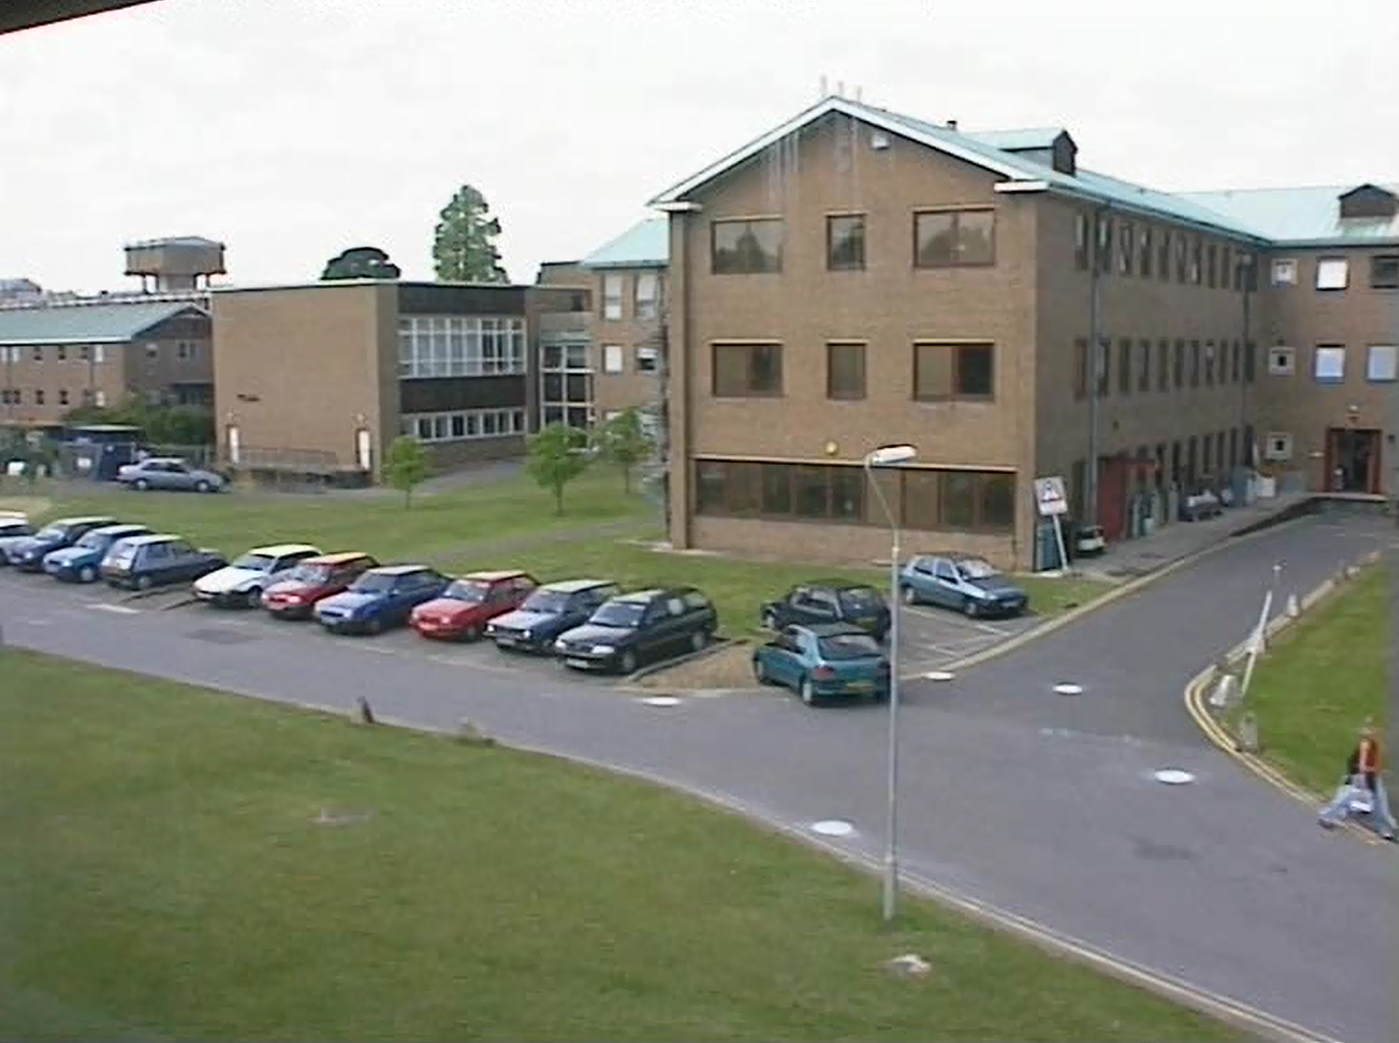
\includegraphics[width=\textwidth]{camReal}
                \caption{Test frame.}
               % \label{fig:gull}
        \end{subfigure}%
        ~ %add desired spacing between images, e. g. ~, \quad, \qquad etc.
          %(or a blank line to force the subfigure onto a new line)
        \begin{subfigure}[b]{0.4\textwidth}
                \centering
                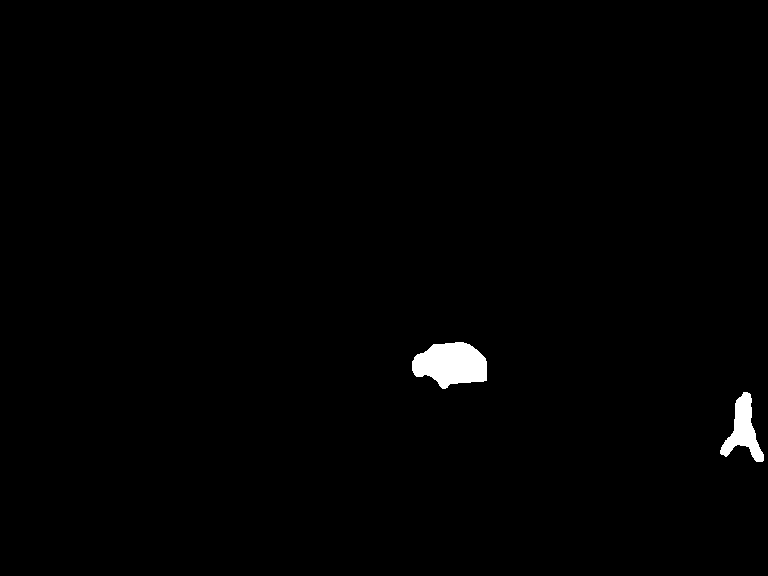
\includegraphics[width=\textwidth]{camGT}
                \caption{Ground truth.}
              %  \label{fig:tiger}
        \end{subfigure}
\caption{The spatial sparsity of foreground. A frame from the PETS data set  \citep{pets2001} and the corresponding foreground in white. In this example, less than 1\% of the frame is foreground, as N=442,368 and K=3862.  }\label{fig:sparse}
\end{figure}

Our method takes a vectorised form of the current frame $\boldsymbol{x_t}$, and acquires compressive measurements $\boldsymbol{y_t}$ of the frame using a Gaussian random matrix $\boldsymbol{\Phi}$. The foreground mask $\boldsymbol{x_t^f} $is then reconstructed by applying a recovery algorithm  to $(\boldsymbol{y_t} - \boldsymbol{y_t^b})$, where $\boldsymbol{y_t^b}$ is a compressed model for the background at time $t$. The silhouette is then thresholded to set any small values to zero, and the non-zero pixels are classified as foreground. 

In order for this method to work well, it is important that a good model of the background is kept updated. Although a static background could be used for short indoor sequences, most real-world video sequences require a dynamic background model. \cite{Piccardi2004a} suggests that a background model should be able to adapt to deal with illumination changes, high frequency repetitive background objects and changes in background geometry. Illumination changes can be separated into gradual changes, or rapid changes. Gradual changes in illumination are mainly due to the light changing throughout the day. Rapid changes in illumination may occur when clouds cover the sun in outdoor scenes or a light being switched on or off in interior scenes. High frequency background objects are mainly found in outdoor footage such as leaves waving in the wind, water rippling or rainy weather. These small movements are actually part of the background so care should be taken to use an algorithm which detects them as such.  Changes in background geometry refers to when part of the background begins to move. Examples of this are very common in real videos, such as a chair being repositioned in a room such as in \cite{toyama1999} or a car driving into a car park as foreground, and then parking therefore becoming part of the background. In this report the background is modelled using an exponentially weighted moving average method as discussed in \cite{Piccardi2004a} and \cite{Cossalter2009}. This is calculated as in equation \eqref{eq:111}.
\begin{equation}
  \label{eq:111}
  \boldsymbol{y_t^b} = \alpha \boldsymbol{y_t} + (1 - \alpha) \boldsymbol{y^b_{t-1}}.
\end{equation}
 where $\alpha \in (0,1)$ is a learning parameter.
This background model was chosen, as it is not computationally heavy, and the single learning parameter $\alpha$ keeps tuning the model simple. The initial background $\boldsymbol{y^b_0}$ is calculated by taking an average of scenes from a training set. If this information is not available it is possible to use only the first frame in the data set, but this may not be as accurate. The background model learning parameter $\alpha$ is tuned so that it is sensitive to the challenges discussed above, specifically to avoid the change in geometry problems. This challenge is especially prominent in the experimentation in Section \ref{sec:results} as the video used is CCTV footage from a car park.   

%Examples may also occur indoors but these are often less prominent.

%The background is modelled using a running average method as discussed in \cite{piccardi2004background} and \cite{Cossalter2009}. 
%This is calculated as in Eq. \eqref{eq:111}.
%\begin{equation}
%  \label{eq:111}
%  \boldsymbol{y_t^b} = \alpha \boldsymbol{y_t} + (1 - \alpha) \boldsymbol{y^b_{t-1}}
%\end{equation}
% where $\alpha$ is a learning parameter.
% The background model learning parameter $\alpha$ has to be tuned well so that it is both sensitive to changes such as cars stopping and starting, but also robust to rapid oscillatory movement such as leaves moving in the wind. The initial background $\boldsymbol{y_0^b}$ is chosen by taking an average a window of training frames, or if there is a lack of training data, it is possible to take the first frame as the initial background.  




\section{Performance Evaluation}\label{sec:results}

The PETS 2001 data set ``camera1''  \cite{pets2001},  is used to compare implementation of the CS$_{\ell_1}$ and CS$_{\text{OMP}}$ algorithms. A quantitative way to characterise the accuracy of these algorithms is to use two performance metrics; precision and recall.  These measures calculate how accurate the segmentation is for a particular frame by comparing the estimated foreground and background with the true values calculated by a hand-segmented ground truth.
% These true values are calculated by segmenting a frame by hand, this frame is known as the ground truth.

In order to quantify how well an algorithm is working, Type I errors and Type II errors must be considered. A Type I error is a false positive (FP), this is experienced when the algorithm classifies a pixel as foreground incorrectly. A Type II error is a false negative (FN), this where the algorithm has neglected to classify a pixel as foreground correctly. If the algorithm works perfectly there will only be True Positives (TP) which are correctly identified foreground pixels and True Negatives (TN), correctly identified background pixels.
Recall is defined as the fraction of correctly identified foreground pixels over the number of ground truth foreground pixels which can be written mathematically as
\begin{equation}
  \label{eq:1}
\text{Recall} = \frac{TP}{TP + FN}. 
\end{equation}
Precision is defined to be the fraction of correctly identified foreground pixels over the number of detected foreground pixels in total, or when written mathematically
\begin{equation}
  \label{eq:2}
\text{Precision} = \frac{TP}{TP + FP}.
\end{equation} 
%\end{definition}

When the recovery algorithms provide an estimate of a foreground mask, the output is not binary but a probabilistic vector. In order to calculate the precision and recall values, a threshold must first be applied to the estimate. Precision-Recall curves can be used to display information relating to the algorithm's performance across a number of thresholds.

In order to have a singular metric to rank the algorithms across a number of thresholds the Area Under Curve (AUC) \citep{Hanley1983} is used. This is equal to the probability that an algorithm  will rank a randomly chosen positive instance higher than a randomly chosen negative one. 
%Although recall and precision can be useful, for ranking performance, it is also good to consider receiver operating characteristic (ROC) curves \cite{Fawcett2006}. ROC curves represent the performance of our classifiers as the foreground threshold is varied.  In order to compare these curves, the Area Under the Curve (AUC) is calculated \cite{Hanley1983}. 

%A value close to 1 implies high recall which means that all of the foreground pixels were correctly identified by the background subtraction algorithm. Recall cannot be used alone as a metric, as even if all of the foreground pixels are correctly detected, this does not give any information on about whether extra pixels have been misclassified as foreground. Hence precision is also used to quantify how accurate the algorithm is. 
%A high precision value implies that of all the pixels classified as foreground, they are also foreground in the ground truth. We can not be sure if we have missed some foreground elements until we consider recall.
%If we wish to rank algorithms in order, it is useful to have one overall measure of the algorithms accuracy. A popular choice in the literature is percentage of correct classifications (PCC). 
%\begin{definition}
%  \label{def:3}
%  Percent of correct classifications (PCC) is defined to be 
%\begin{equation}
%  \label{eq:3}
% \frac{TP+TN}{TP + TN + FP + FN},
%\end{equation}
%where TP, TN, FP and FN are defined as above. 
%\end{definition}
%Although PCC can be useful for ranking performance, it is important to not just rely on one metric. It is possible for a background subtraction technique to fail to detect any foreground in the test frame giving a recall value of 0, but the PCC could still be very high if the algorithm correctly identifies all of the true negatives. This is a good example of why metrics cannot be solely relied on, and reinforces the importance of visually analysing the output as well as considering metrics.
%The ROC AUC is equivalent to the probability that our algorithm will rank a randomly chosen positive instance higher than a randomly chosen negative one. 
%CS$_{\text{OMP}}$ struggles with respect to both performance metrics, whilst CS$_{\ell_1}$ gives a poor recall value despite good precision. Both algorithms struggle with recall which indicates that the algorithms missclassify many true foreground pixels as background. This could be due to a failure when the foreground occupies a very small area but some noise is also accidentally identified by background subtraction algorithms. This could perhaps be avoided by incorporating a more stable background subtraction algorithm, or applying a detection threshold which only attempts to reconstruct foreground if it takes up at least a certain percentage of the entire frame. This detection threshold would hopefully also lower computational complexity, but could be very difficult to tune correctly. 
%NOISE etc
%\begin{table}[h]
%  \centering
%  \begin{tabular}{c|c|c|c}
%    & Precision & Recall & AUC \\ \hline 
%$\ell_1$ &0.9144 &0.1845 &0.9940 \\
%OMP & 0.4012&0.0623 &0.9877 \\
%  \end{tabular}
%\caption{Performance metrics} \label{tab:1}
 %0.4012     0.0623     0.9755     0.9877     0.9144     0.1845     0.9807     0.9940
%\end{table}

\begin{table}[ht!]
\caption{CS$_{\ell_1}$ and CS$_{\text{OMP}}$ segmentation for 3 test scenes ($N = 4096, M = 2048, \alpha = 0.05$). }
\centering
\begin{tabular}{cccc}
\parbox[top]{30mm}{Original frame.} & 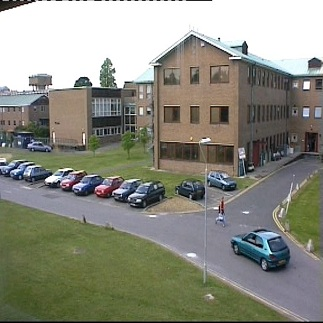
\includegraphics[width=30mm]{1}& 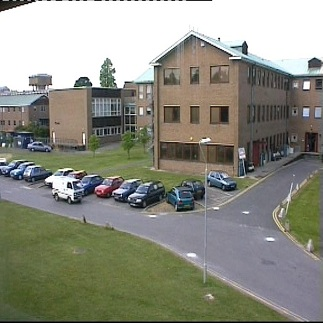
\includegraphics[width=30mm]{2} & 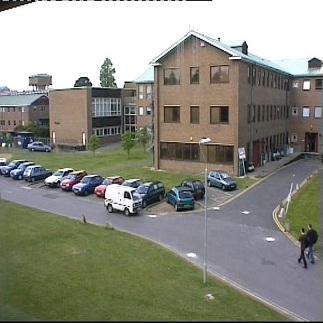
\includegraphics[width=30mm]{3} \\
\parbox[top]{30mm}{Ground truth.} & 
\includegraphics[width=30mm]{GTB}& 
\includegraphics[width=30mm]{GTD} & 
\includegraphics[width=30mm]{GTE} \\
\parbox[top]{30mm}{CS$_{\ell_1}$.} & 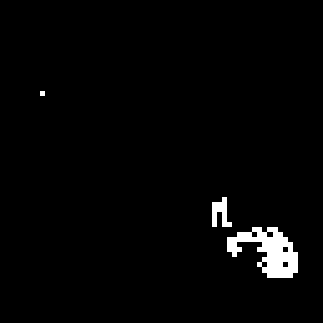
\includegraphics[width=30mm]{1l}& 
\includegraphics[width=30mm]{2l} & 
\includegraphics[width=30mm]{3l} \\
\parbox[top]{30mm}{CS$_{\text{OMP}}$.} & 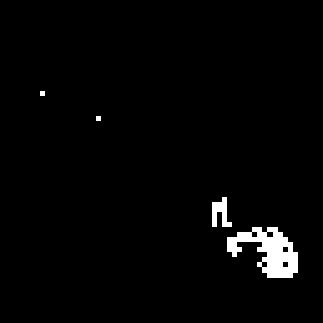
\includegraphics[width=30mm]{1o}& 
\includegraphics[width=30mm]{2o} & 
\includegraphics[width=30mm]{3o} \\
\end{tabular}
\label{tab:gt}
\end{table}

%\begin{table}[ht!]
%\caption{Ground Truth, L1 and OMP segmentation for 5 test scenes ($N = 4096, M = 2048, \alpha = 0.05$). }
%\centering
%\begin{tabular}{cc}
% 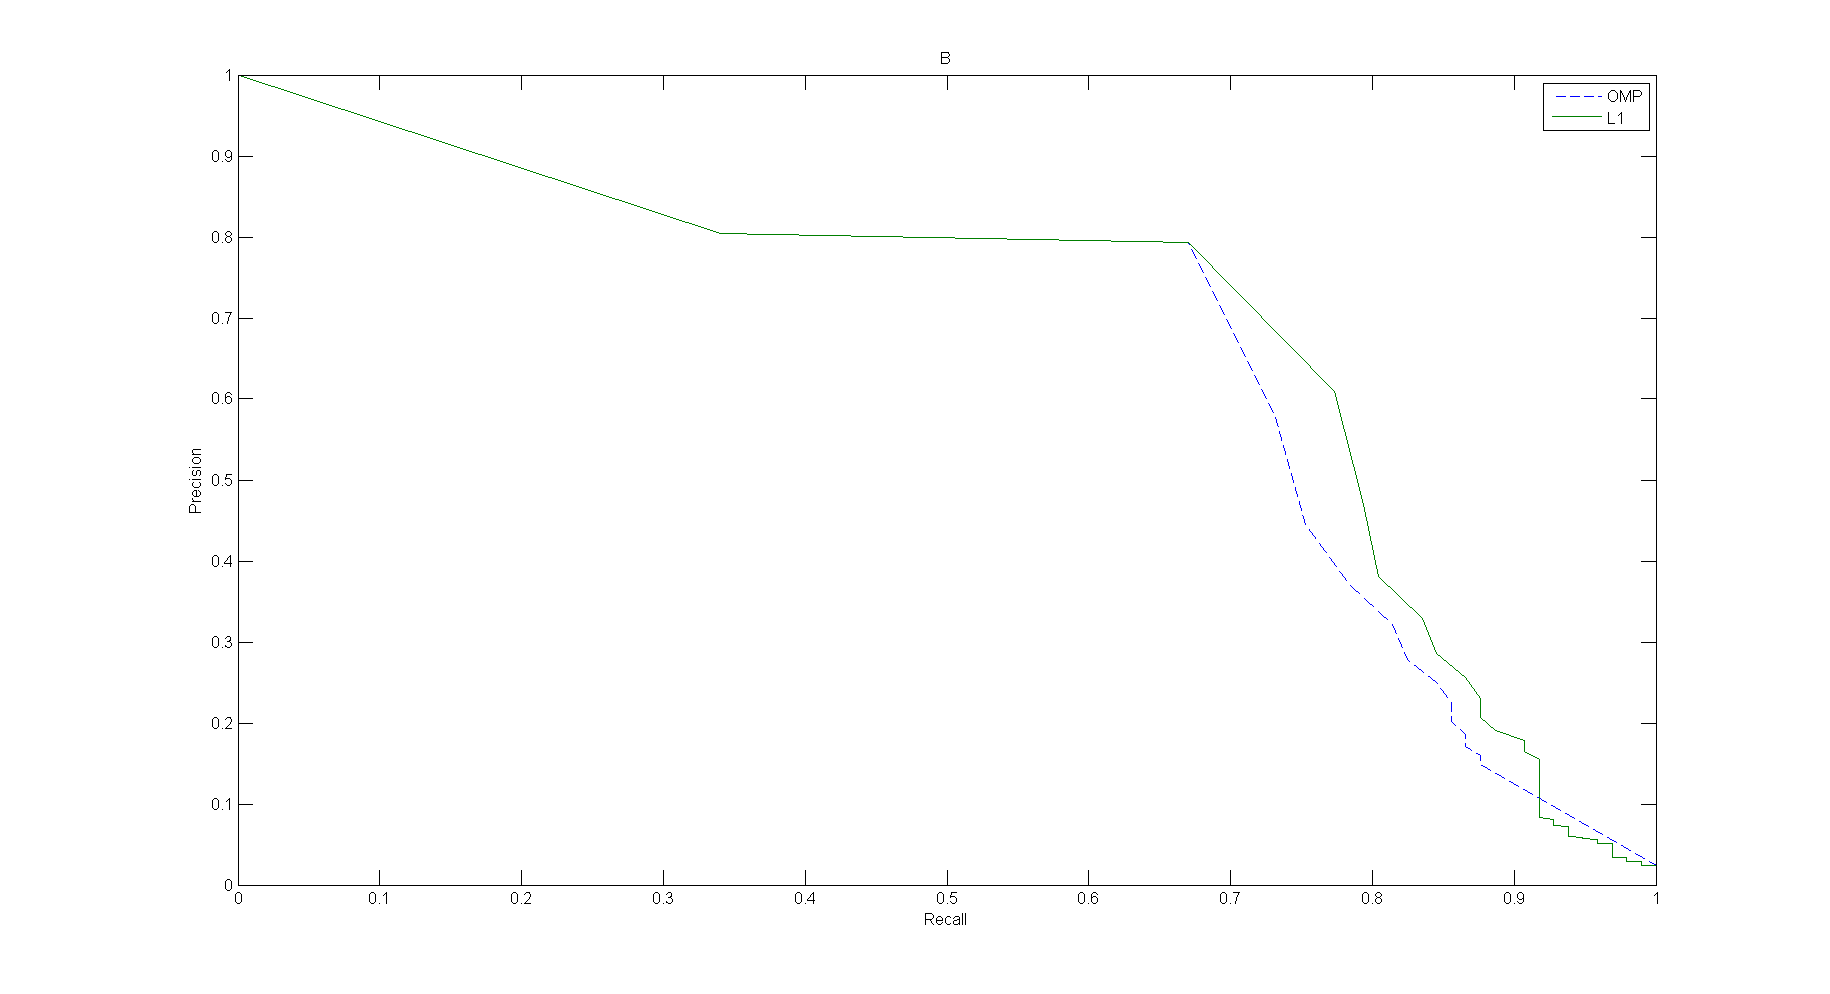
\includegraphics[width=35mm]{Bpr}&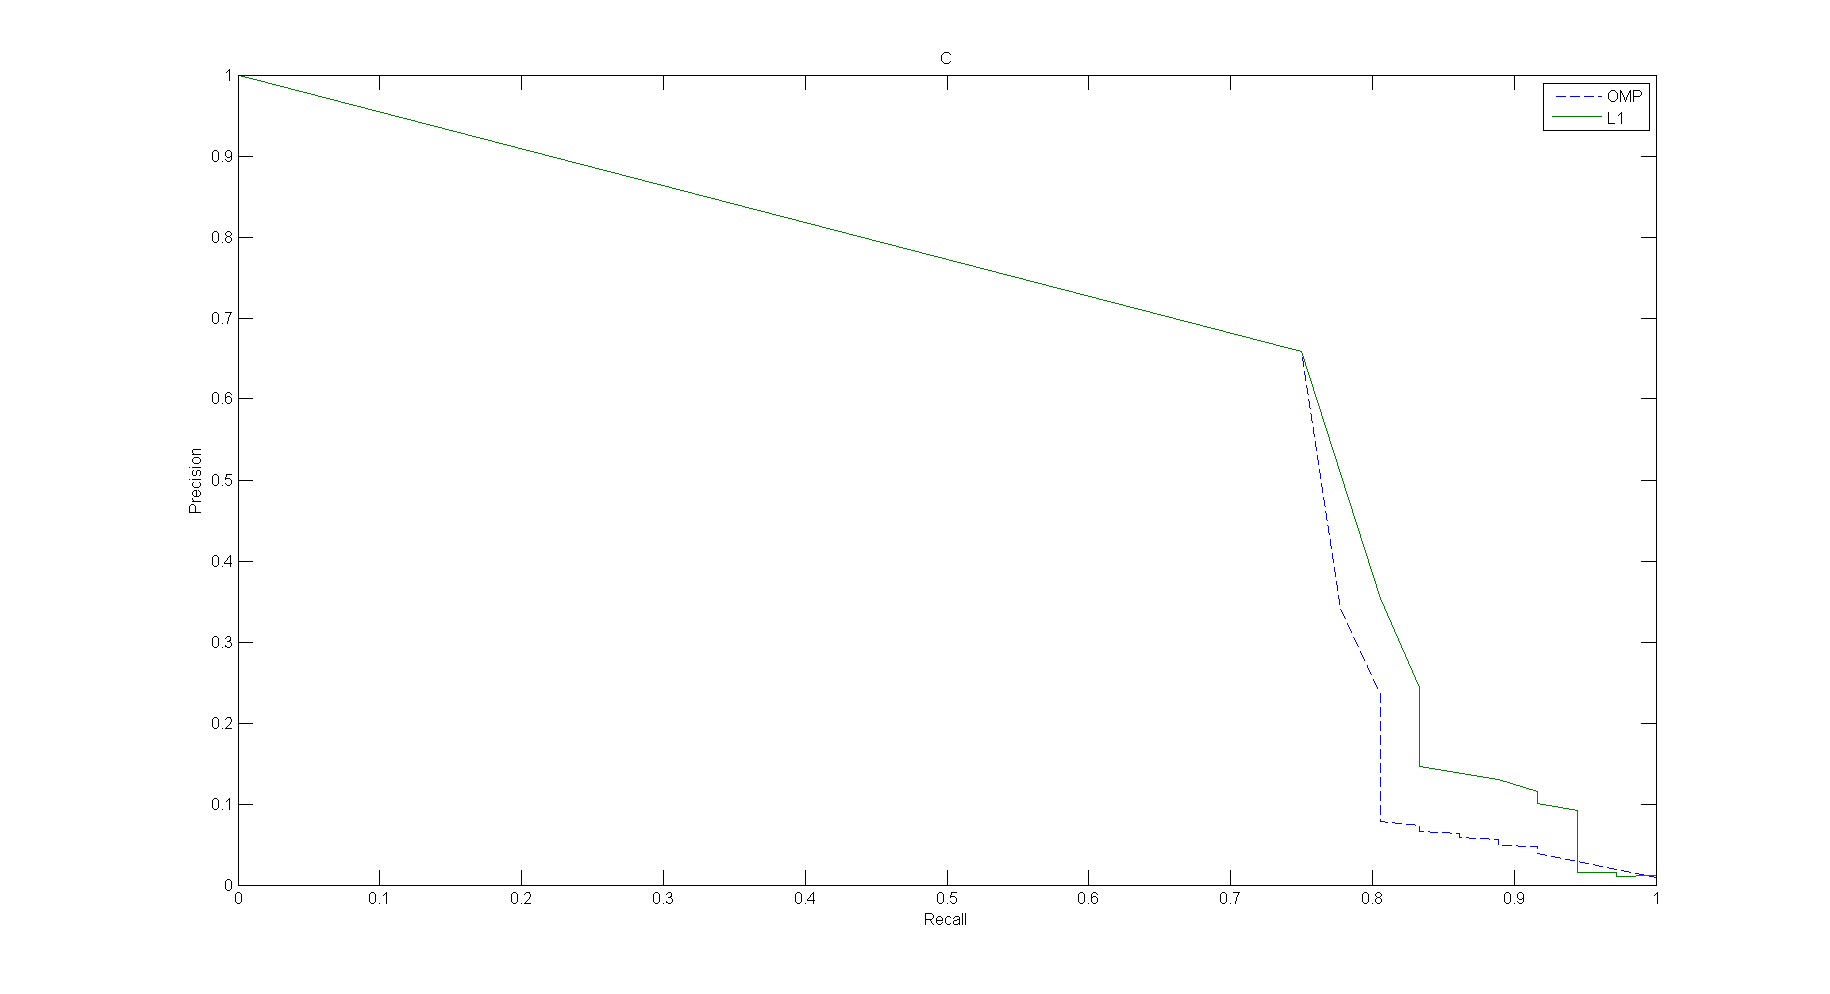
\includegraphics[width=35mm]{Cpr} \\
% 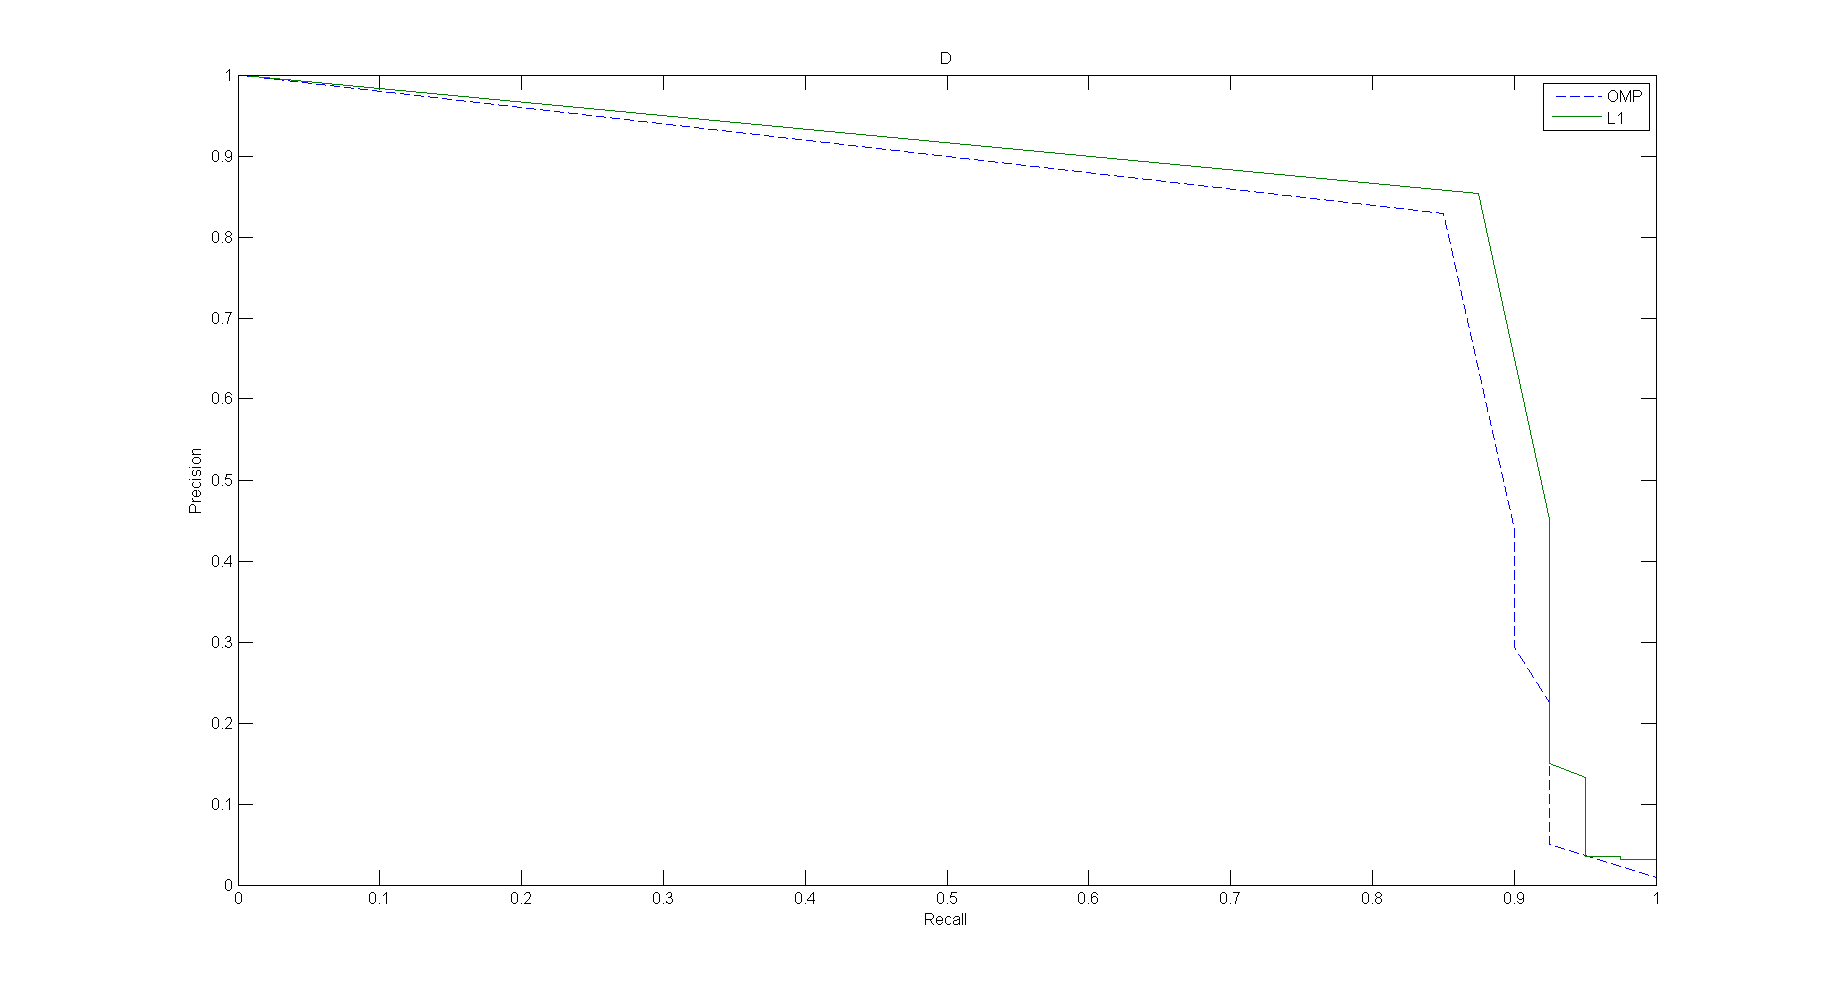
\includegraphics[width=35mm]{Dpr}&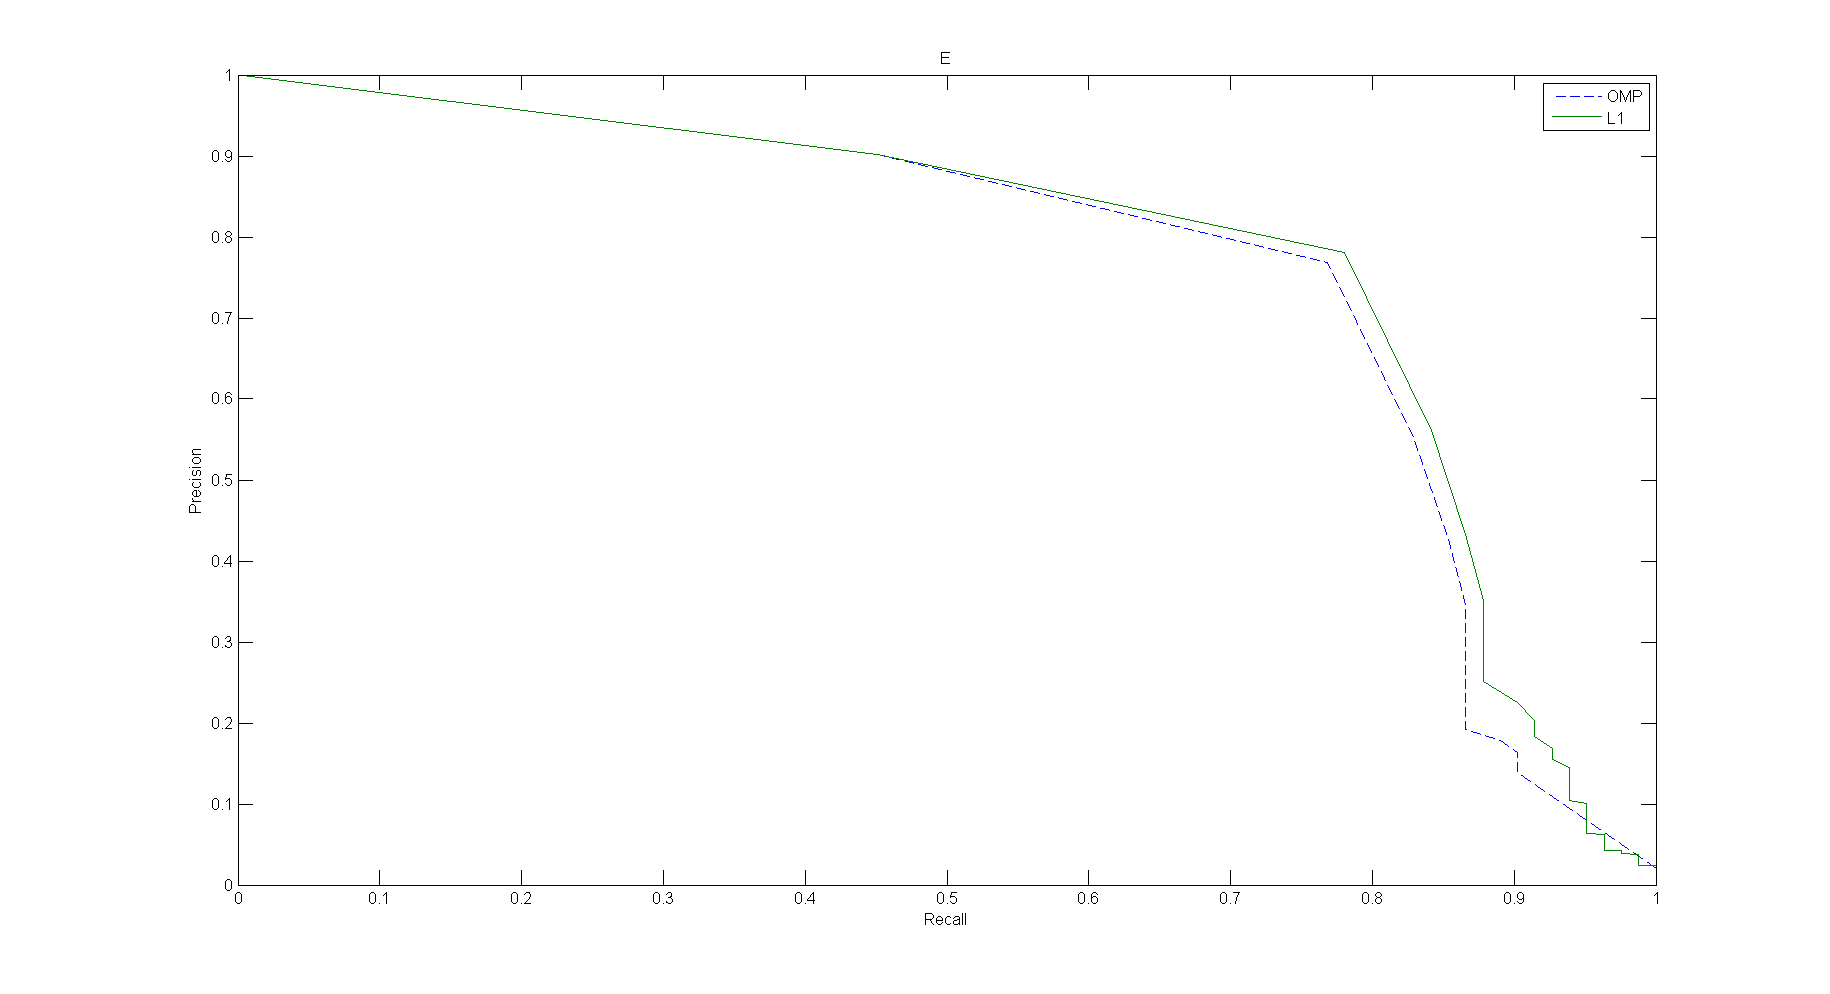
\includegraphics[width=35mm]{Epr} \\
%\end{tabular}
%\label{tab:gt}
%\end{table}
%Both algorithms struggle to fill in the foreground  entirely. This could be due to the threshold being set too low or perhaps some blob processing could be applied in order to improve this. Note that in the third image, both algorithms perform badly. In this scene a car is slowing and stopping in order to park, and so perhaps the background model is not adapting quick enough.

Foreground masks for three test frames can be found in Table \ref{tab:gt}. These images have been thresholded so any value above $0.004$ is classed as foreground and everything else is set to background. The performance of both algorithms is very similar, although the Precision-Recall curves in Figure \ref{fig:precrec} imply that CS$_{\ell_1}$ may be slightly outperforming CS$_{\text{OMP}}$ across the different thresholds. 

\begin{figure}[H]
  \centering
  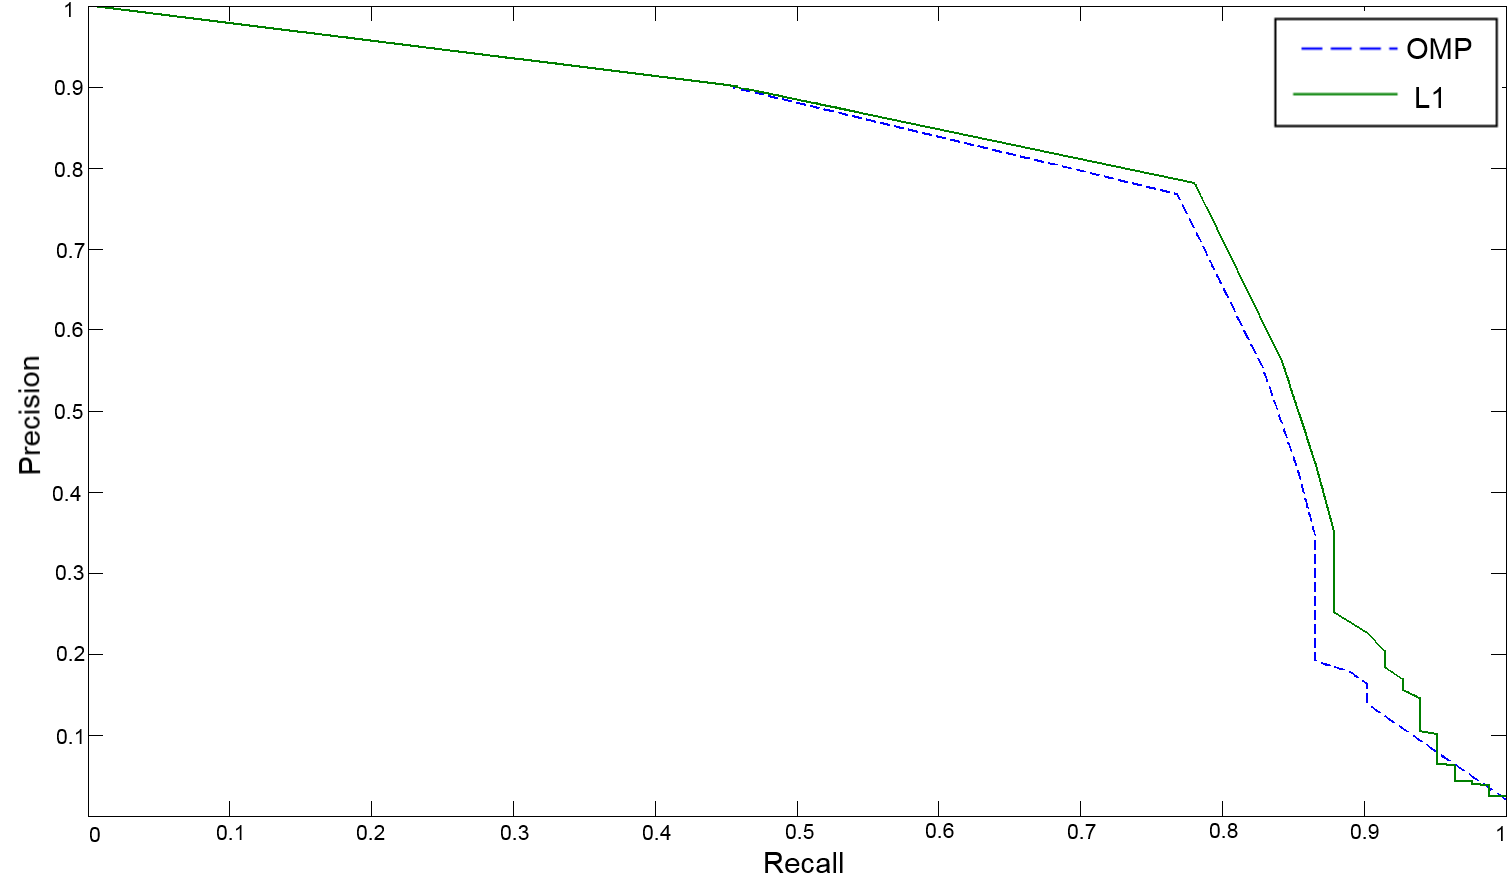
\includegraphics[width = 9cm]{Epr_EDIT}
  \caption{Precision-Recall Curves for the 3rd test frame.}
  \label{fig:precrec}
\end{figure}

The effect of the stopping criterion for the orthogonal matching pursuit can be seen in Figure \ref{fig:omp}.

\begin{figure}[H]
  \centering
  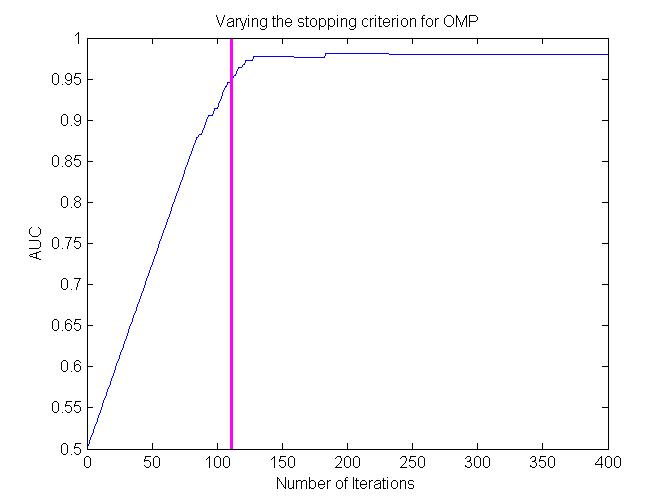
\includegraphics[width = 9cm]{varyingSComp}
  \caption{Selection of the stopping criterion for OMP.}
  \label{fig:omp}
\end{figure}

 The stopping criterion is increased between $1$ and $400$ and the AUC is calculated at each stage. As discussed in Section \ref{sec:greedy-algorithm}, the selection of the stopping criterion can have an impact on the results; too small and it will underestimate the size of the foreground, too large and computational expense will increase greatly with no noticeable performance improvement. This can be seen in the steep increase of performance in Figure \ref{fig:omp}. Note that as the number of iterations reaches approximately the ``true'' sparsity $111$ of the foreground, the performance increases. Ideally, the stopping criterion should be as small as possible to minimise the computational cost, but not at the expense of poor segmentation. 

Another consideration is the effect of the choice of $M$ on recovery accuracy. Ideally the number of $M$ should be as small as possible in order to keep computations cost low, whilst still retaining a good enough quality of detection to suit the application, whether it be tracking, classification etc. Figure \ref{fig:sr} shows the performance of both algorithms as the compression ratio $\frac{M}{N}$ increases, with respect to AUC. There is a sharp rise in performance as the compression ratio increases to 20\%, and as we approach a compression rating of 30\%, both algorithms are performing very well. Note that CS$_{\ell_1}$ is constantly outperforming CS$_{\text{OMP}}$ in this experiment over all compression ratios.

\begin{figure}[H]
  \centering
  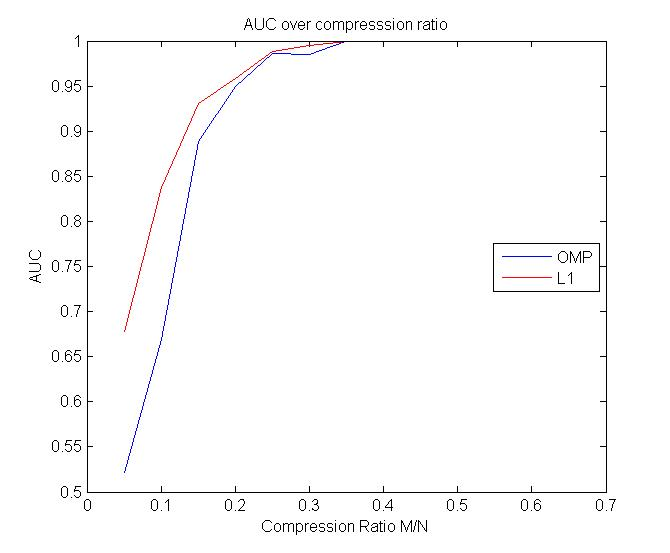
\includegraphics[width = 9cm]{AUCcompressionRatio}
  \caption{AUC over Sparsity Ratio.}
  \label{fig:sr}
\end{figure}


\section{Conclusions and Further Work}\label{sec:conclusions}
This paper presents results about the effects of different compressive sensing recovery algorithms on background subtraction for surveillance footage. In our experimentation basis pursuit outperforms orthogonal matching pursuit across the foreground thresholds, although it is hard to distinguish them from foreground masks alone.  The effect of the stopping criterion for OMP was seen to have a large impact on performance, which indicates the necessity for adaptive iterations in order to cope with varying sparsity in a video. It is also indicated that ideal boundaries for the compression ratio $\frac{M}{N}$ are between $25 - 35\%$.  One important question to address in future is, is it possible to incorporate more prior information about surveillance footage and use this to aid the recovery process? In current methods, there is a failure to use the natural structural properties of foreground, such as the expectation of foreground to take the shape of a person or vehicle. Structured sparsity has not been well explored in the compressive sensing background subtraction literature although a start in this area has been made by \cite{La2006} and \cite{Duarte2008}. Future work seeks to apply a clustering method to these background subtraction algorithms and to build in a natural way to allow the sparsity constraint in the algorithms to vary between frames. 



%---------------- COMMENT FOR IMPORTING ----------------------
%\pagebreak											%Comment for importing
%\bibliographystyle{plainnat}		%Comment for importing
%\bibliography{References}				%Comment for importing
%\end{document}									%Comment for importing
%-------------------------------------------------------------

